

\section{Methodology}
\label{sec:method}
We begin by providing a formal description of a multi-head self-attention layer (Section~\ref{sec:pre}).
Building on this, we theoretically revisit the foundational principles of existing Top-$k$ eviction methods by introducing an $L_1$ eviction loss metric (Section~\ref{sec:revisiting}).
Inspired by theoretical findings, we propose a simple yet effective strategy for adaptive budget allocation, which is proven to outperform traditional uniform budget allocation (Section~\ref{sec:optimizing}).
We further demonstrate its compatibility with existing Top-$k$ eviction methods (Section~\ref{sec:integration}) and present an efficient implementation (Section~\ref{sec:imp}).





\subsection{Preliminaries}
\label{sec:pre}
LLMs operate through an autoregressive generation process, where each step relies on the last token to predict the next one. Let $X\in \mathbb{R}^{n \times d}$ represent the embedding matrix containing all tokens in the sequence, and let $x \in \mathbb{R}^{1 \times d}$ be the embedding of the last token used as input at the current time step.
Using the notation system from ~\cite{liu2023dejavucontextualsparsity} with
$h$ attention heads, we provide a formal description of one multi-head self-attention layer.
For each head $i \in [1, h]$, the transformation matrices $W_i^Q$, $W_i^K$, $W_i^V \in \mathbb{R}^{d \times d_h}$ map token embeddings to their respective Query, Key, and Value states, while the final output matrix $W_i^O \, \in \mathbb{R}^{d_h \times d}$ transforms the intermediate result to the output hidden states. At each time step, the previous KV cache elements of head $i$ are initialized as:
$
	K_i = XW_i^K,V_i=XW_i^V
$.
Then, the embedding of input token $x$ is mapped to its respective  Query, Key, and Value states  for each head, and the previous KV cache is updated accordingly:
{\small
\begin{equation}
	q_i = xW_i^Q,k_i = xW_i^K,v_i = xW_i^V
    \: and \:
	K_i = Cat[K_i:k_i],V_i=Cat[V_i:v_i]
\end{equation}
}
Finally, the output $y \in \mathbb{R}^{1 \times d}$ is computed using the attention weights $A_i \in \mathbb{R}^{1 \times n}$ as follows\footnote{The scaling factor $\sqrt{d_h}$ is omitted for simplification.}:
{\small
\begin{equation}
	y = \sum_{i \in [1, h]} A_i V_i W_i^O \: \text{where} \: 	A_i = \text{softmax}(q_{i}K_i^{T})
\end{equation}
}
\subsection{Theoretical Foundation: Revisiting Top-$k$ Methods with Bounded Eviction Loss}
\label{sec:revisiting}
Top-k eviction methods typically presuppose the stability of critical cache elements during future generation process, to facilitate cache eviction~\cite{H2o,SnapKV,PyramidInfer,PyramidKV}. SOTA methods~\cite{SnapKV,PyramidInfer,PyramidKV} commonly leverage query states of a series of tokens within an observation window to calculate observed attention weights with past KV cache elements. These weights, combined with Top-k selections, approximate the identification of cache elements critical in subsequent generations.



For ease of presentation, we assume a window size of 1, implying the eviction procedure relies solely on the attention weights $A$ between the past cache elements and the query state of the last token for the detection of critical cache elements. A set of indicator variables $\left\{\mathcal{I}_i \in \mathbb{R}^{1 \times n}\right\}$\footnote{Given that the first dimension of $\mathcal{I}_i$ is 1, $\mathcal{I}_i^j$ is used to simplify the notation for $\mathcal{I}_i(1, j)$. Similarly, $A_i^j$ follows the same notation.} represent the eviction decision, with allocated budgets $\left\{B_i\right\}$ for all heads $\{i \in [1,h]\}$, where $B = \sum_{i \in [1, h]} B_i$ is the overall budget for one attention layer:
\begin{equation}
\text{Eviction Decision:} \quad	\mathcal{I}_i^j  =
	\begin{cases}
		1 	\quad	  \text{Retain  $K_i^j \: \text{and} \: V_i^j$,   }\\
		0   \quad    \text{Evict  $K_i^j \: \text{and} \: V_i^j$},\\
	\end{cases}
\end{equation}
where $\mathcal{I}_i^j$ indicates whether the $j\text{th} \in [1, n]$ KV cache element in $K_i,V_i \in \mathbb{R}^{n \times d_h}$ is evicted for head $i$.
Thus, only a budget size $B_i$ of cache elements is retained for head $i$: $\sum_{j \in [1,n]} \mathcal{I}_i^j = B_i$.
%, and the overall budget for one attention layer is $B = \sum_{i \in [1, h]} B_i$.
Then, the post-eviction output $\hat{y}$ of multi-head self-attention mechanism is:
 \begin{equation}
 	\hat{y} = \sum_{i \in [1, h]} \hat{A}_i V_i W_i^O,
 	\text{where} \: \hat{A}_i  = \text{softmax}(-\infty \odot ( \textbf{1} - \mathcal{I}_i) + q_iK_i^{T}),
 \end{equation}
and $\odot$ denotes element-wise multiplication.



The degradation in generation quality after cache eviction stems from changes in the attention output. We quantify the eviction loss as the $L_1$ distance between the pre- and post-eviction outputs of the self-attention mechanisms:
\begin{equation}
	L_1 \: \text{Eviction Loss} = ||y-\hat{y}||_1
\end{equation}
Utilizing the row norm of the matrix, we derive an upper bound $\epsilon$ for the $L_1$ Eviction Loss in Theorem \ref{thm:bound}. For a detailed proof, please refer to Appendix \ref{apdx:prof_bound}.
\begin{theorem}
	\label{thm:bound}
	  The $L_1$ eviction loss  can be bounded by $\epsilon$:
	{\small
	\begin{equation}
	L_1 \: \text{Eviction Loss} \leq \epsilon = 2hC - 2C\sum_{i\in [1, h]}\sum_{j \in [1,n ]} \mathcal{I}_i^jA_i^j
	%  \\  &\text{given allocated budgets}  \left\{B_i\right\} \notag
	\end{equation}	
	}
	%&where \: C =  \notag
	where $C=Max\left\{\lVert V_iW_i^O\rVert_{\infty} \right\}$ is a constant number, representing the max row norm .
		\vspace{-0.2cm}
\end{theorem}



Essentially, existing cache eviction methods are equivalent to minimizing the upper bound $\epsilon$, as defined in Theorem~\ref{thm:bound}. One such method, Top-$k$ cache eviction method~\cite{H2o,SnapKV,PyramidInfer,PyramidKV} stands out as a prominent approach, designed to selectively retain the most critical cache elements by  prioritizing those with the highest attention weights. Specifically, the Top-$k$ eviction decision is formulated as :
	\begin{equation*}
		\text{Top-$k$ Eviction Decision } \:
		\mathcal{I}_i^{*j}  =
		\begin{cases}
			1 	\:	  \text{ if $A_i^j \in \text{Top-$k$}(A_i, k= B_i)$,   }\\
			0 \: \text{Evict  $K_i^j \: \text{and} \: V_i^j$}.\\
		\end{cases}
	\end{equation*}
{
This approach ensures that each head $i$ retains only the top $B_i$ critical cache elements based on attention weights $A_i^j$, evicting the rest. In Theorem \ref{thm:upper_bound}, we prove that the Top-$k$ eviction decision $\left\{ \mathcal{I}^*_i \right\}$ achieves the tightest upper bound $\epsilon^*$, establishing its effectiveness, under given budget allocation $\left\{B_i\right\}$. For a detailed proof, please refer to Appendix \ref{apdx:proof_upper_bound}.
}


\begin{theorem}
	\label{thm:upper_bound}
 The Top-$k$ cache eviction $\left\{ \mathcal{I}^*_i \right\}$ minimizes the upper bound $\epsilon$ of $L_1$ eviction loss, resulting in $\epsilon^*$:
		\begin{equation}
		\text{Top-k eviction decision} \:	\left\{ \mathcal{I}^*_i \right\} = \argmin_{\left\{ \mathcal{I}_i \right\}} \epsilon  \:\: and \:\:
			\epsilon^*= \min_{\left\{ \mathcal{I}_i \right\}} \epsilon = 2hC - 2C\sum_{i\in [1, h]}\sum_{j \in [1, n]}^{A_i^j \in \text{Top-$k$}(A_i,k=B_i)} A_i^j
		\end{equation} 
\end{theorem}

{
Theorems \ref{thm:bound} and \ref{thm:upper_bound} establish the theoretical basis for Top-$k$ eviction methods under any given budget allocation $\left\{B_i\right\}$.
In the sequel, we show how an adaptive strategy can further minimize $\epsilon^*$, outperforming uniform budget allocation (i.e., $\left\{B_i = B/h\right\}$).
}



\subsection{Optimizing Top-$k$ Methods with Adaptive Budget Allocation}
\label{sec:optimizing}
		\begin{algorithm}[H]  
%			\small  
			\caption{Ada-KV: Adaptive Budget Allocation}  
			\label{alg:allocation}  
			\textbf{Input}: Total budget: $B$; Attention weights for head $i$: $\left\{A_{i}\right\}$ \\
			\textbf{Output}: Allocated budgets  $\left\{B^*_i \right\}$  
			\begin{algorithmic}[1]  
				\STATE Concatenate attention weights across heads $A=\text{Cat}\left(\{A_i\}\right)$  
				\STATE Select top $B$ weights from $A$: Top-$k$($A,k=B$)  
				\STATE Count number of selected weights for each head $i$: $\{f_i\}$  
				\STATE Set the allocated budgets as $\{B^*_i = f_i\}$ \\
				\textbf{Return} allocated budgets $\{B^*_i\}$  
			\end{algorithmic}  
		\end{algorithm}  

Here, we propose the first adaptive budget allocation strategy for Top-$k$ eviction methods in Algorithm \ref{alg:allocation}, designed to further minimize the upper bound $\epsilon^*$ in Theorem \ref{thm:upper_bound}.
It begins by identifying the $B$ largest attention weights across all heads within a single layer. Based on the frequency of  selection in each head, the strategy dynamically determines the  budget allocation $ \{ B^*_i \} $. Thereby, attention-sparse heads, where most attention weights are concentrated on only a few cache elements, are assigned a smaller budget. The saved budget is  reallocated to attention-dispersed heads with more widespread concentration patterns. Thus it effectively adapts to the distinct attention patterns inherent to each head. Below, we further demonstrate the superiority of this strategy theoretically and empirically in subsequent sections.







\textbf{Theoretical Advantages of Adaptive Allocation.}
Given the adaptive budget allocation  $\{ B^*_i\}$, the upper bound associated with the Top-$k$ eviction decision $\left\{\mathcal{I}_i^* \right\}$  is expressed as  $\epsilon^{**}$:
\begin{equation}
	\epsilon^{**}=  2hC - 2C\sum_{i\in [1, h]}\sum_{j \in [1, n]}^{A_i^j \in \text{Top-$k$}(A_i,B^*_i)} A_i^j
\end{equation}
Theorem~\ref{thm:better} demonstrates that the adaptive budget allocation achieves the minimum upper bound  $\epsilon^{**}$  compared to any other allocation strategy, including the commonly used uniform allocation.  A detailed proof is provided in Appendix \ref{apdx:proof_better}.
\begin{theorem}
	\label{thm:better}
	The adaptive budget allocation  $\{ B^*_i\}$, derived from Algorithm~\ref{alg:allocation} achieves the minimal upper bound $\epsilon^{**}$ for loss associated with Top-$k$ eviction strategies:
		$
			\epsilon^{**} = \min_{\left\{B_i\right\}} \epsilon^{*}
	$
	\vspace{-0.2cm}
\end{theorem}
Although a lower upper bound does not strictly guarantee reduced eviction loss, it is generally a key objective in algorithm design, as optimizing a tighter bound typically leads to better results.



\textbf{Empirical Evidence for Adaptive Allocation.}
Empirically, the adaptive budget allocation described in Algorithm~\ref{alg:allocation} assigns larger budgets to dispersed heads and conservatively adjust budgets for sparse heads. This approach aligns well with the significant variation in attention concentration across heads, as shown in Figure~\ref{fig:accu_weights}.  By adjusting the head-wise budget, this strategy effectively reduces practical eviction loss. Figure~\ref{fig:loss_comparation} provides a detailed visualization, showing that adaptive budget allocation consistently reduces practical eviction loss across most samples under the same cache budget. These results demonstrate the effectiveness of the proposed method in real-world scenarios.



\begin{figure*}[t]  
	\centering  
	\vspace{-0.3cm}
	% 左侧算法  
	\begin{minipage}[t]{0.60\textwidth}  
		\vspace{0pt}  
		\begin{algorithm}[H]  
			\small  
			\caption{Ada-SnapKV/Ada-Pyramid in One Layer}  
			\label{alg:ada_snap}  
			\textbf{Input}: total budget $B$, tokens in observation window $X^{win} \in \mathbb{R}^{win * d}$, cache in observation window $\left\{K_i^{win},V_i^{win}\right\}$, cache outside observation window $\left\{K_i,V_i\right\}$\\
			\textbf{Output}: retained cache  $\hat{K}_i,\hat{V}_i$  
			\begin{algorithmic}[1]  
				\FOR{$i \gets 1$ to $h$}  
				\STATE $Q_i^{win} = X^{win}W_i^Q$  
				\STATE $\bar{A_i} =softmax(Q_i^{win} K_i^T)$  
				\STATE $\bar{A_i} =\bar{A_i} .maxpooling(dim=1).mean(dim=0)$  
				\ENDFOR  
				\STATE $B = B - winsize \times h$  
				\STATE Derive budget allocation  $\left\{B_i^*\right\}$ using Algorithm \ref{alg:allocation}($B,\left\{\bar{A}_i\right\} $)  
				\STATE Safeguard $\left\{B_i^*\right\} = \alpha \times \left\{B_i^*\right\} + (1-\alpha) \times (B/h)$  
				\STATE Determine the Top-$k$ eviction decision $\left\{\mathcal{I}_i^* \right\}$ based on $\left\{B_i^*\right\}$  
				\STATE Select $\left\{\hat{K}_i,\hat{V}_i\right\}$ from $\left\{K_i,V_i\right\}$ according to { $\left\{{\mathcal{I}_i^*}\right\}$} 		  
				\STATE  $\left\{\hat{K}_i,\hat{V}_i\right\} = \text{Cat}(\left\{\hat{K}_i,\hat{V}_i\right\},\left\{K_i^{win},V_i^{win}\right\})$\\
				\textbf{Return}  retained cache $\hat{K}_i,\hat{V}_i$  
			\end{algorithmic}  
		\end{algorithm}  
	\end{minipage}  
	\hfill  
	% 右侧图形  
	\begin{minipage}[t]{0.38\textwidth}  
		%\begin{figure}
			\vspace{0pt}  
			\begin{subfigure}[b]{\linewidth}  
				\centering  
				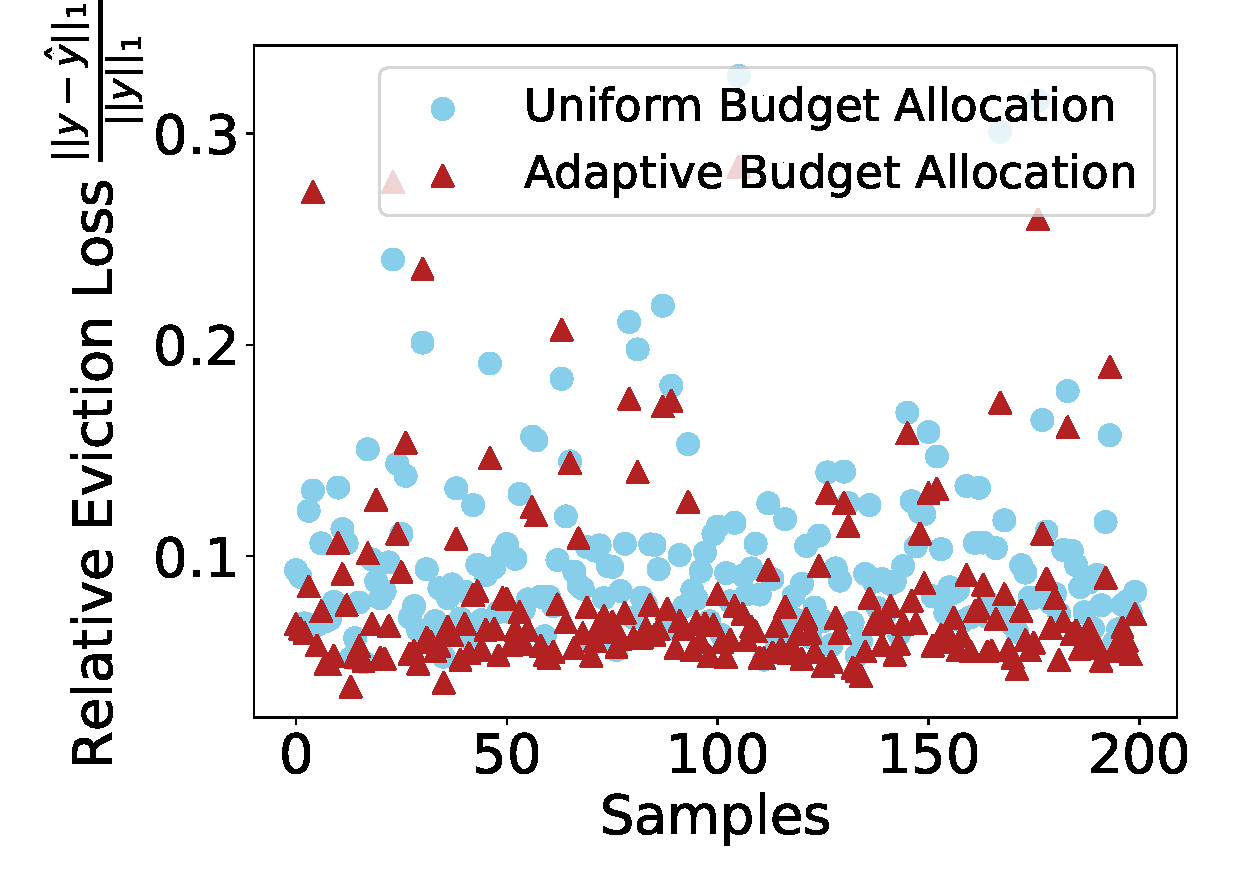
\includegraphics[width=0.7\linewidth]{./Figures/eviction_loss_budget05.pdf}  
				\vspace{-0.2cm}  
				 \captionsetup{labelformat=empty} 
				\caption{\small $B$ = 20\% cache size}    
			\end{subfigure}  
			\begin{subfigure}[b]{\linewidth}  
				\centering  
				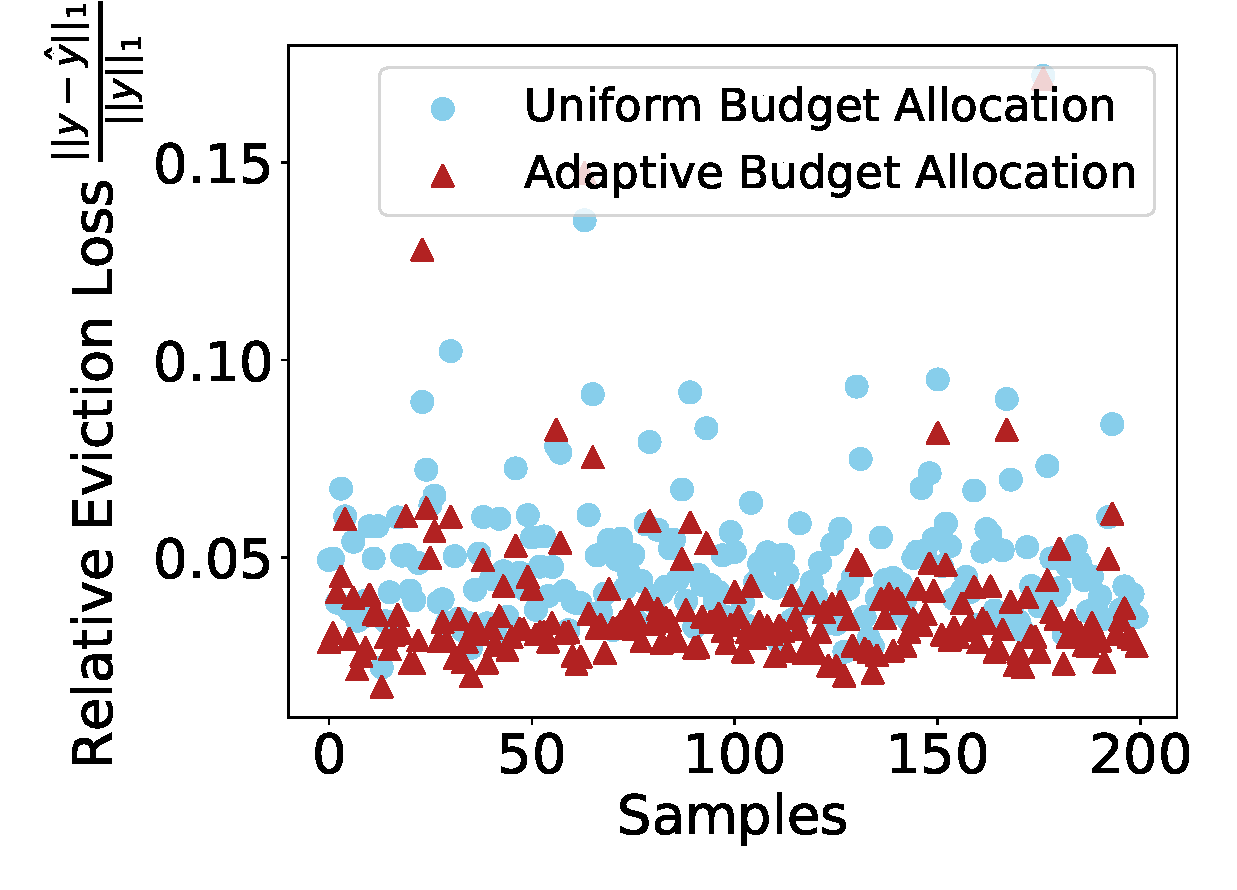
\includegraphics[width=0.7\linewidth]{./Figures/eviction_loss_budget10.pdf}  
				\vspace{-0.2cm}  
				 \captionsetup{labelformat=empty} 
				\caption{\small $B$ = 40\% cache size}  
				\vspace{-0.2cm}  
			\end{subfigure}    
			\caption{Adaptive allocation yields lower practical eviction losses (Llama-3.1-8B-Instruct on Qasper Dataset).}
			\label{fig:loss_comparation}  
			\vspace{-0.3cm} 
		%\end{figure}
	\end{minipage}
	\vspace{-0.3cm}  
\end{figure*}








\subsection{Integration into Existing Cache Eviction Methods}
\label{sec:integration}
We demonstrate the Plug-and-Play compatibility of Ada-KV strategy with two SOTA methods, SnapKV and Pyramid, by integrating it into their existing Top-$k$ eviction frameworks to create enhanced versions: Ada-SnapKV and Ada-Pyramid.
Both SnapKV and Pyramid utilize tokens $X^{win} \in \mathbb{R}^{winsize * d}$ from a recent observation window (typically size 32) to identify and evict the less crucial elements in past KV cache.
SnapKV excels under larger budget scenarios, while Pyramid is optimized for constrained budget conditions.
This is because Pyramid uses a pyramidal budget distribution across attention layers via pre-set hyperparameters, prioritizing shallower layers. Thus, for a given layer with a total budget of $B$, their eviction algorithms are identical. However, both methods allocate budgets evenly across all heads within one layer.

Incorporating our adaptive allocation, as outlined in Algorithm \ref{alg:ada_snap}, we modify these methods to better manage budget allocation at the head level.
This integration occurs prior to the eviction process in each layer, where our strategy adaptively adjusts budget allocations based on the observed attention weights among heads, as shown in Line 7. Overall, they first calculate the observed attention weights $\bar{A}_i$ of past cache elements using the query states within the observation window. A max pooling layer processes these weights to preserve essential information~\cite{SnapKV}, followed by a Top-$k$ selection of past cache elements outside the observation window.
These selected elements, along with others within the observation window, are retained, while the rest are evicted.
Moreover, we introduce a safeguard hyper-parameter, $\alpha$ (defaulted to 0.2), to prevent the allocation of excessively small budgets to highly sparse heads, thereby enhancing fault tolerance for presupposed critical stability~\cite{SnapKV,H2o}.
%  of  elements

\subsection{Implementation of Computation under Adaptive Budget Allocation}
\label{sec:imp}
\textbf{Variable-length Attention with Variable-sized Cache Elements.} Adaptive allocation improves cache eviction quality but introduces challenges for efficient computation due to variable-sized cache elements across attention heads. We found that the variable-length FlashAttention technique~\cite{dao2022flashattention,dao2023flashattention}, widely adopted in many inference frameworks for continuous batching~\cite{kwon2023efficient}, could support efficient computation under adaptive allocation. To further enable this technique, we implement a flattened cache storage layout that concatenates the caches of all attention heads within a layer into a single tensor structure. This layout, combined with a custom CUDA kernel, enables efficient cache update operations. As demonstrated in Section \ref{sc:exp_efficiency}, these components work in synergy to maintain computational efficiency under adaptive allocation, comparable to that of conventional FlashAttention.




\textbf{Compatibility with Group Query Attention.}
Existing SOTA LLMs like Llama~\cite{llama3} and Mistral~\cite{jiang2023mistral}, have  employed Group Query Attention (GQA)~\cite{GQA} technique to reduce KV cache sizes.
However, existing cache eviction methods, such as SnapKV and Pyramid, lack GQA compatibility, redundantly replicating grouped KV caches across heads.
We implement a simple GQA-compatible  mechanism that uses the mean attention weight within each group as the selection criterion, eliminating redundancy. This enables SnapKV, Pyramid, and their adaptive variants---Ada-SnapKV and Ada-Pyramid---to achieve significant cache size reductions, such as a 4x reduction in Llama-3.1-8B.


